\clearpage
\section{Exemplos de análise de dados}
\label{sec:analise}

Os dois exemplos usam a base de notas do guia. Primeiro contamos as notas ausentes. Depois comparamos as notas disponíveis por curso.

\subsection{Quantas notas estão faltando em cada curso?}

A contagem de notas ausentes usa \codigo{df}, a tabela original da Seção \ref{sec:ler}. Em um agrupamento, \codigo{size} conta todas as linhas e \codigo{count} conta os valores presentes na coluna. A diferença dá o número de notas ausentes. Dividir essa diferença pelo total do curso dá a proporção de registros sem nota.

\begin{exemplo}
cobertura = df.groupby("curso")["nota"].agg(
    total="size", com_nota="count"
)
cobertura["sem_nota"] = cobertura["total"] - cobertura["com_nota"]
cobertura["pct_sem_nota"] = (
    100 * cobertura["sem_nota"] / cobertura["total"]
).round(1)
print(cobertura)
\end{exemplo}

No gráfico empilhado, \codigo{bottom} faz a barra de notas ausentes começar no topo da barra de notas presentes. A altura total mostra o número de registros.

\begin{exemplo}
import matplotlib.pyplot as plt

fig, ax = plt.subplots(figsize=(6.3, 3.5), layout="constrained")
ax.bar(cobertura.index, cobertura["com_nota"],
       color="#19476B", label="Com nota")
ax.bar(cobertura.index, cobertura["sem_nota"],
       bottom=cobertura["com_nota"], color="#D69865",
       label="Sem nota")
ax.set(title="Registro de notas por curso", xlabel="Curso",
       ylabel="Quantidade de registros", ylim=(0, 8))
ax.legend(loc="upper center", ncol=2, frameon=False)
plt.show()
\end{exemplo}

\noindent\begin{minipage}{\linewidth}
\centering
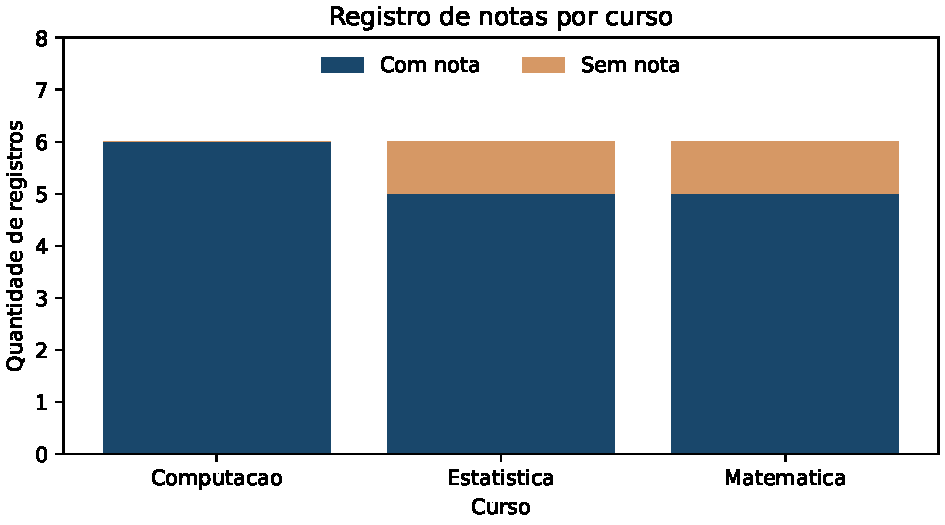
\includegraphics[width=0.66\linewidth]{figuras/notas-ausentes.pdf}

\raggedright
Estatística e Matemática têm uma nota ausente cada, ou \(16{,}7\%\) dos seus seis registros. Computação tem as seis notas. A causa das ausências depende de informações adicionais.
\end{minipage}

\needspace{34\baselineskip}
\subsection{Como as notas se distribuem por curso?}

A comparação usa as notas observadas em \codigo{df\_validas}, da Seção \ref{sec:ausentes}. \codigo{ax.boxplot()} recebe uma sequência de notas por curso. O eixo horizontal indica quantas observações entraram em cada grupo.

\begin{exemplo}
import matplotlib.pyplot as plt

notas_por_curso = []
rotulos = []
for curso, notas in df_validas.groupby("curso")["nota"]:
    notas_por_curso.append(notas.to_numpy())
    rotulos.append(f"{curso}\n(n={len(notas)})")

fig, ax = plt.subplots(figsize=(6.3, 3.6), layout="constrained")
ax.boxplot(notas_por_curso,
           medianprops={"color": "#19476B", "linewidth": 2})
ax.set_xticks(range(1, len(rotulos) + 1), rotulos)
ax.set(title="Notas por curso", ylabel="Nota")
plt.show()
\end{exemplo}

\noindent\begin{minipage}{\linewidth}
\centering
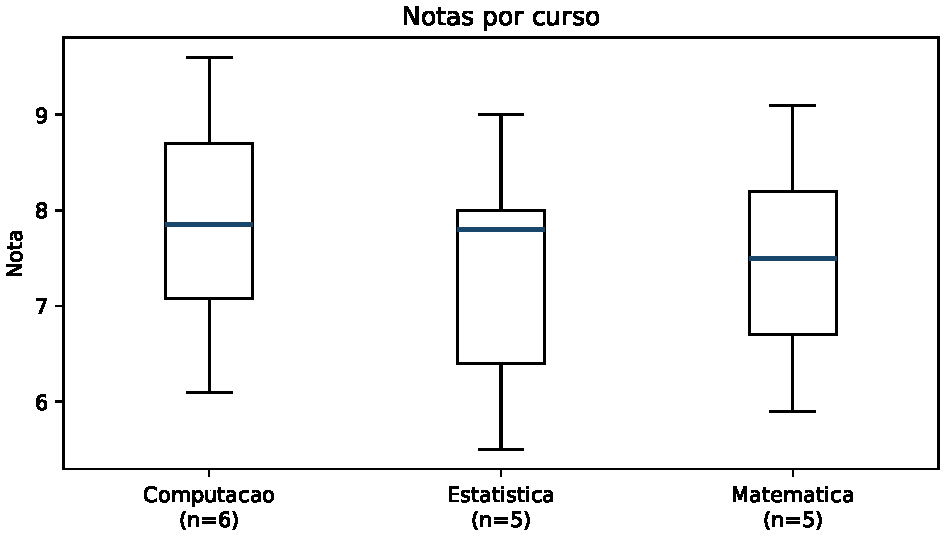
\includegraphics[width=0.69\linewidth]{figuras/notas-por-curso.pdf}

\raggedright
As medianas são \(7{,}85\), \(7{,}80\) e \(7{,}50\) em Computação, Estatística e Matemática, respectivamente. As caixas se sobrepõem e cada grupo tem apenas cinco ou seis notas. A comparação descreve esse conjunto simulado.
\end{minipage}

\needspace{6\baselineskip}
\subsection{Outras perguntas que viram gráficos}

\noindent\begin{tabularx}{\linewidth}{@{}>{\raggedright\arraybackslash}p{0.34\linewidth}>{\raggedright\arraybackslash}X>{\raggedright\arraybackslash}X@{}}
\toprule
\textbf{Pergunta} & \textbf{Como organizar os dados} & \textbf{Gráfico} \\
\midrule
Em que turno há mais atendimentos? & Contar atendimentos por turno. & Barras com uma categoria por turno. \\
Qual é o tempo de espera mais comum? & Reunir os tempos individuais, em minutos. & Histograma com intervalos de mesma largura. \\
Como o consumo de energia mudou durante o ano? & Somar o consumo de cada mês, em kWh. & Linhas com os meses na ordem do calendário. \\
O tempo de estudo e a nota variam juntos? & Usar os dois valores do mesmo participante e identificar seu curso. & Dispersão com um marcador por curso e legenda. \\
\bottomrule
\end{tabularx}\par
